%% USPSC-Anexos.tex
% ---
% Inicia os anexos
% ---

% Imprime uma página indicando o início dos anexos

\begin{anexosenv}
% ---
%\partanexos
\noindent \chapter{Exemplo de anexo}
\vfill
\clearpage
% ---
Elemento opcional, que consiste em um texto ou documento não elaborado pelo autor, que serve de fundamentação, comprovação e ilustração, conforme a ABNT NBR 14724. \cite{nbr14724}.



\noindent\chapter{Acentuação (modo texto - \LaTeX)}
\vfill
\clearpage
\begin{figure}[H]
	
	\caption{\label{fig_anexob}Acentuação (modo texto - \LaTeX)}
	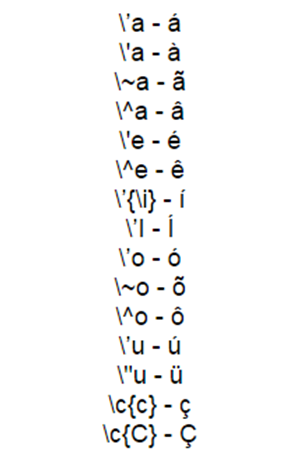
\includegraphics[scale=1.0]{imagens/USPSC-AcentuacaoLaTeX.png} \\
	%Fonte: \citeonline{comandos}
	Fonte: \citefonte{comandos}

\end{figure}

\end{anexosenv}
